\documentclass{article}
\usepackage{graphicx} % Required for inserting images
\usepackage{hyperref} % Required for hyperlinks

\begin{document}

\maketitle
\newpage
\section{Transfer Function}
Low Pass:
\[
\frac{{v_{\text{in}} - x}}{{R_1}} + \frac{{v_0 - x}}{{R_2}} + (v_0 - x)C_2s = 0
\]
\[
\frac{{v_0 - x}}{{R_2}} + v_0C_1s = 0
\]
Solving, we have
For the Low Pass filter, the transfer function \( H(s) \) is given by:
\[ H(s) = \frac{1}{{c_1 c_2 R_1 R_2 s^2 + s c_1 (R_1 + R_2) + 1}} \]

This equation describes the relationship between the input (\( v_{\text{in}} \)) and output (\( v_0 \)) signals in the Low Pass filter circuit.

% Inserting an image
\begin{figure}[ht]
  \centering
  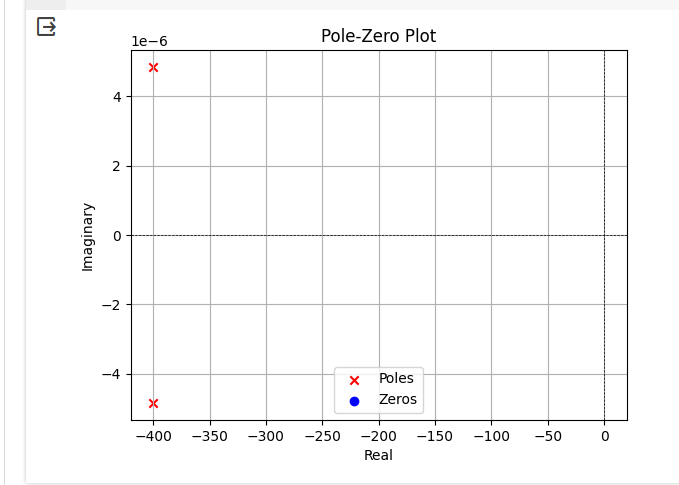
\includegraphics[width=0.7\textwidth]{Screenshot from 2023-11-15 17-44-45.png} % Replace 'Screenshot_from_Low_Pass_Plot.png' with the actual file name and path
  \caption{Pole Zero Plot for Low Pass Filter}
  \label{fig:your_image}
\end{figure}
\newpage
Band Pass:
\[
v_{\text{in}} - iR_1 - \frac{i}{C_1s} - \frac{i}{C_2s(1 + C_2s)} = V_0
\]
\[
i = \frac{v_{\text{in}}}{R_1+ \frac{1}{c_1s}} 
\]
on solving we get 
\[
H(s) = -\frac{c_1}{c_2} \cdot \frac{1}{(R_1C_1s + 1)(R_2C_2s + 1)}
\]
This equation describes the relationship between the input (\( v_{\text{in}} \)) and output (\( V_0 \)) signals in the High Pass filter circuit.

% Inserting an image
\begin{figure}[ht]
  \centering
  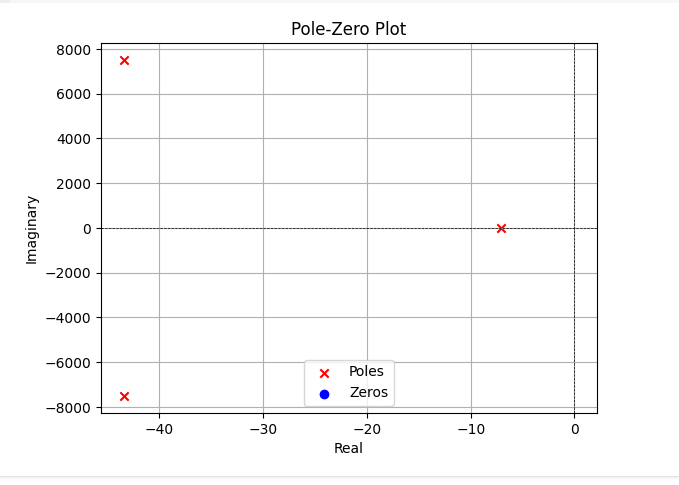
\includegraphics[width=0.7\textwidth]{Screenshot from 2023-11-15 18-08-17.png} % Replace 'Screenshot_from_High_Pass_Plot.png' with the actual file name and path
  \caption{Pole Zero Plot for High Pass Filter}
  \label{fig:your_image_high_pass}
\end{figure}

As seen in both the plots, the poles have negative real value, thus the design is stable. 


For the Python code generating these plots, refer to 

\url{https://colab.research.google.com/drive/1koj8sK5V5i7SiOVdr0mSccGSmV1wG-v0?authuser=1#scrollTo=-b5ql538-t14}.
\end{document}
